\chapter{General Post Office and Head Office Postmarks of the Cape of Good Hope}
 


The first datestamps specifically designating the Cape 
Town General Post Office were circular (GPO 1 to 4) and were in use 
from about 1881. They measured from 22 to 25 mm in diameter, 
with the letters G.P.O. at the top of the circle and "Cape Town" 
underneath. The letters vary in height from 3 to 4 mm. During 1891 
a new datestamp was brought into use (G.P.O 5).
\begin{marginfigure}
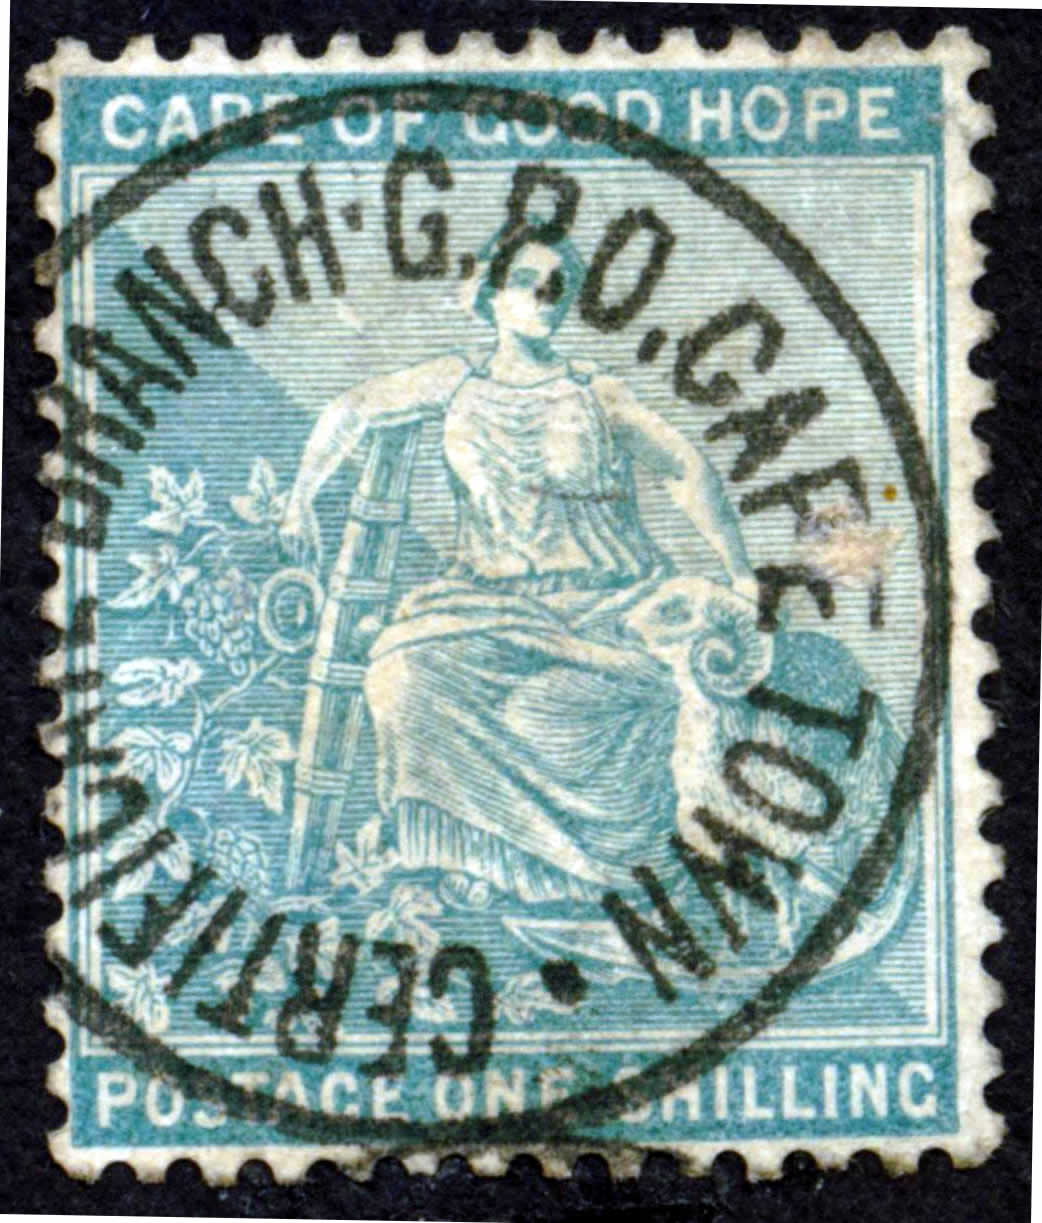
\includegraphics[width=1.0\textwidth]{../cape-of-good-hope/GPO/Certificate.jpg}
\end{marginfigure}


During 1891, a new postmark was brought into use (GPO 5). 
This incorporated the letters C.G.H. at the bottom of the circle. 
It is found in various diameters ranging from 22 mm to 25 mm. 
In 1895 a datestamp (GPO 6) was issued with the wording 
'GPO Cape Town' in the upper portion of the postamark and 
words 'Cape Town' at the bottom.
Branches and Departmental Postmarks

Various Departments of the Post office used different 
cancellations and postmarks. In some towns there were head 
post offices as well as branches. Departments amongst others 
were the Record Branch, the Poste Restante, the Certificate 
department and the Money Order Office. These incorporated 
postmarks as shown in GPO 7 to GPO 13. These normally 
incorporated additional wording or abbreviations to designate 
the Department or particular branch.
Head Post Offices
 

 

H.P.O Postmarks (GPO 8) were used to distinguish the Head Post Office 
from branches. The letters H.P.O appear at the bottom of the circle. 
In Cape Town the letters G.P.O. (General Post Office) were used instead.

\subsection{Poste Restante}

\ph[width = .80\textwidth]{../cape-of-good-hope/GPO/post-restante.jpg}{ }


Poste Restante, the Department where mail was kept until 
called for used two different postmarks. One with lettering 
3 mm high and another one with lettering 2.5 mm (See GPO 9 and GPO 10).

\subsection{The Record Branch}

Postmarks denoting the Record Branch of the General Post 
Office of the Cape of Good Hope are found on letters and 
documents that required to be recorded by that Department. 
These are sometimes also found on letters, but this was 
only to indicate that the subject matter mentioned in the 
letters had been dealt with by the Records Branch. It did 
not perform any postal function.
 
\subsection{The Postmaster General's Handstamp}

\ph[width = .80\textwidth]{../cape-of-good-hope/GPO/Postmarks-Record-Branch.jpg}{ }

In the Postmaster-General's office a handtamp (GPO 11) was used to 
datestamp letters and documents. It must be noted that as with the 
Record Branch handstamps, these were to be used for datestamping 
documents and not envelopes. Sometimes it is found cancelling fiscal 
stamps on documents.

 

 

 

 

 
 
                     